\documentclass[a4paper,12pt,obeyspaces,spaces,hyphens]{article}

\usepackage{agenda}
\usepackage{colortbl}
\usepackage{xcolor}
\usepackage{palatino}
\usepackage{calc}

\hypersetup{pdftitle={TE5009 Embedded Software},
  pdfauthor={Leo Sandoval}}

\begin{document}

\thispagestyle{fancy}

\setlength{\arrayrulewidth}{0.8pt}

\begin{center}
\LARGE
TE5009 Embedded Software\\
\large
10-day session
\end{center}
\vspace{1cm}

\small
\newcolumntype{g}{>{\columncolor{fedarkblue}}m{4cm}}
\newcolumntype{h}{>{\columncolor{felightblue}}X}

\arrayrulecolor{lightgray} {
  \setlist[1]{itemsep=-5pt}
  \begin{tabularx}{\textwidth}{|g|h|}
    {\bf Title} & TE5009 Embedded Software Course \\
    \hline

    {\bf Overview} &
    Part I.   Principles of Modern Embedded Systems \par
    Part II.  Embedded Systems Architecture \par
    Part III. Embedded Systems Operation \par
    Part IV.  Embedded Linux System Development \par
    Part V.   Embedded Linux Application Development \\
    \hline

    {\bf Duration} & {\bf Ten} sessions - 30 hours (3 hours per session).
    \newline 50\% of lectures, 50\% of practical labs.  \\
    \hline
  \end{tabularx}

  \begin{tabularx}{\textwidth}{|g|h|}
    {\bf Required equipment} &
    \begin{itemize}
    \item PC computers with at least 2 GB of RAM, and Ubuntu/Debian Linux
    installed in a {\bf free partition of at least 50 GB. Using Linux
      in a virtual machine is not recommended}, because of issues
    connecting to real hardware.
    \item {\bf Connection to the Internet}.
    \end{itemize} \\
    \hline

    {\bf Materials} & Print and electronic copies of presentations and
    labs.
    \newline Electronic copy of lab files.\\
    \hline

  \end{tabularx}}
\normalsize

\feagendatwocolumn
{Hardware}
{
  \begin{itemize}
    \item Freescale i.MX6 based {\bf Sabre SDB} Board (provided by the
      instructor)
  \end{itemize}
}
{}
{
  \begin{center}
    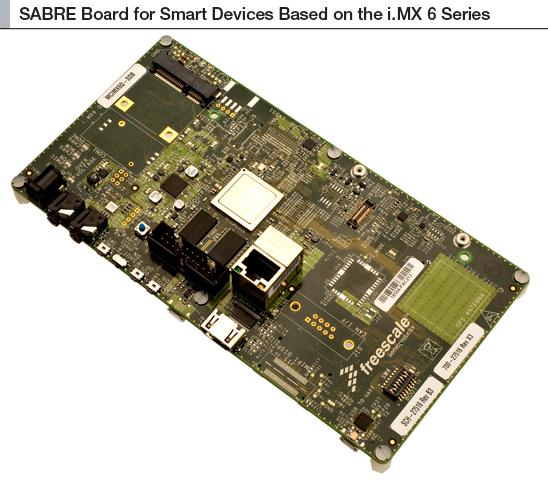
\includegraphics[height=5cm]{agenda/RDIMX6SABREBRD_BD.jpg}
  \end{center}
}

\feagendatwocolumn
{Hardware}
{
  \begin{itemize}
    \item  Freescale i.MX6 based HummingBoard Board (Provided by the students,
      optional)
  \end{itemize}
}
{}
{
  \begin{center}
    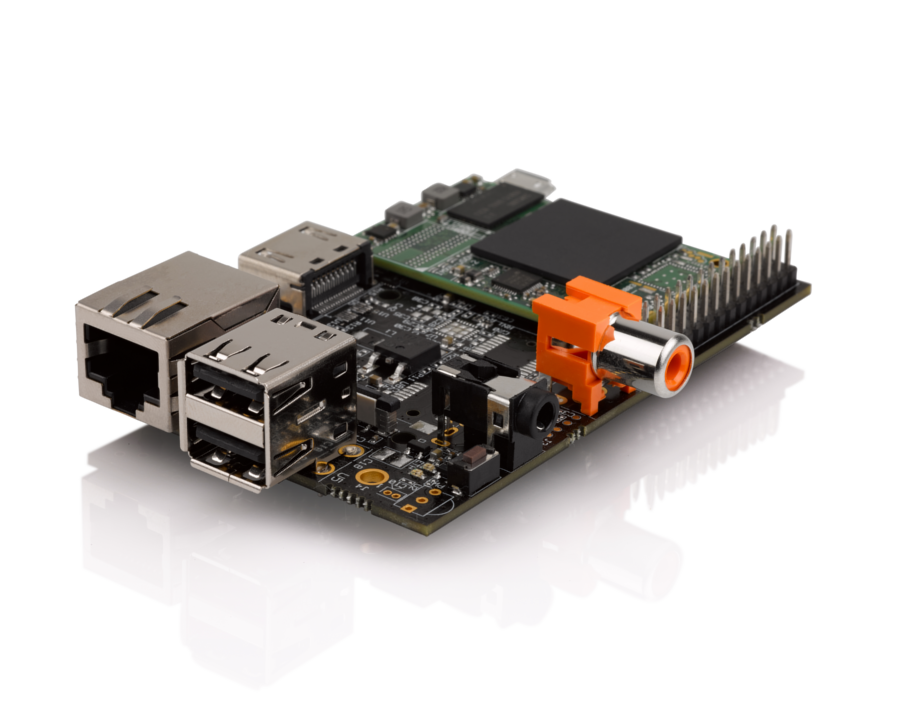
\includegraphics[height=5cm]{agenda/HummingBoard-i2.png}
  \end{center}
}

\section{Part I}

\feagendaonecolumn
{Lecture - Principles of Modern Embedded Systems}
{
  \begin{itemize}
    \item Landscape
    \item Attributes
    \item Future
  \end{itemize}
}

\section{Part II}

\feagendaonecolumn
{Lecture - Embedded Systems Architecture}
{
  \begin{itemize}
    \item SoC
    \item Memory
    \item Communications Interfaces
    \item Pins
    \item Freescale i.MX6 Application Processors
    \item Freescale i.MX Sabre Board for Smart Devices
    \item i.MX based Humming Board
  \end{itemize}
}

\section{Part III}

\feagendatwocolumn
{Lecture - Embedded Systems Operation}
{
    \begin{itemize}
      \item Toolchain
      \item i.MX6 Platform SDK
      \item Bootloader
      \item Linux Kernel
      \item Filesystem
    \end{itemize}
}
{Lab - Toolchain}
{
  \begin{itemize}
    \item Compile a toolchain
    \item Compile the i.MX6 Platform SDK
    \item Patch the SDK and run a test
 \end{itemize}
}

\section{Part IV}

\feagendatwocolumn
{Lecture - Embedded Systems Operation}
{
  \begin{itemize}
    \item Open Source
    \item System Building
  \end{itemize}
}
{Lab - Debian and Yocto Proyect}
{
  \begin{itemize}
    \item Create a Debian System
    \item Build a Freescale image with Yocto Project
 \end{itemize}
}

\section{Part V}

\feagendatwocolumn
{Lecture - Embedded Linux Application Development}
{
  \begin{itemize}
    \item Application development
    \item Source management
    \item Debugging and analysis tools
    \item Development environments
  \end{itemize}
}
{Lab - Multimedia Acceleration}
{
  \begin{itemize}
    \item Clone, branch and compile a github MM repo
    \item Compare SW and HW processing
 \end{itemize}
}

\end{document}
